\documentclass{sig-alternate}
\usepackage{etoolbox}
\makeatletter
\patchcmd{\maketitle}{\@copyrightspace}{}{}{}
\makeatother

\usepackage[caption=false]{subfig}
\usepackage{verbatimbox}
\providecommand{\e}[1]{\ensuremath{\times 10^{#1}}}
\usepackage{enumitem}




\begin{document}

\title{Randomized Optimization, Unsupervised Learning, and Dimensionality Reduction}
\subtitle{Writeup for Assignment 02 - CS 6741}

\author{
\alignauthor
Magahet Mendiola
}
\date{}

\maketitle
\begin{abstract}
An empirical analysis of planning and reinforcement learning algorithms in the context of marchov decision processes.
\end{abstract}

\section{Planning Metrics}
A number of simple metrics were used to evaluate the performance of our planning algorithms. These include the number of iterations and elapsed time required to find the optimal utility values for each state. However, the goal of planning is to find the optimal policy for an MDP, and not the optimal set of utility values. Therefore, we can also compare how long it takes each to find the optimal policy for each state.

There is also the rate at which a policy converges toward the optimum. This can be seen with the hamming distance between the current policy and the optimal policy at each iteration. If a partial plan can be created quickly, it may be good enough for practical use on the MDP.

Another derivation of the hamming distance metric is the time/iterations required to find the policy which will successfully guide a deterministic agent to the goal state. The idea behind this metric is that there may be many states that are never visited. Running value or policy iteration until enough of the states have optimal policies to guide the agent could greatly reduce planning time.

Creating a planning algorithm with this stopping criteria would be similar to q-learning in regards to limiting exploration. It would also be similar to a* path finding, with search areas radiating omni-directionally from non-zero reward states.


\section{Grid Worlds}

Each algorithm was tested against contrived gridworld type MDPs. These worlds were setup to accentuate the strengths and weaknesses of each algorithm. They also illustrate the impact of rewards, discounts, and  and to point out opportunities for modifications to each.

\subsection{Discount Grid}

This grid world, titled Discount Grid \cite{project3}, is useful for illustrating the effects of utility discounting, transition function probabilities, and state rewards on optimal policies. It includes two terminal states with positive rewards (+1 closer, +10 farther) and five negative terminal states at the bottom edge of the grid. This setup allows us to explore what set of problem and solution parameters affect the goals defined by an optimal policy.

Figure~\ref{discount-default} shows the resulting values of the MDP after running value iteration with a $\gamma$ of 0.9 and a reward of 0 in all the non-terminal states. The transition probabilities are 0.8 for desired action and a combined 0.2 for all orthogonal movements. In this case, the policy directs the agent to seek out the farther, higher valued, terminal state. It also avoids the high penalty cliff except when the alternative is moving into the lower reward terminal state.

\begin{figure}[!htbp]
    \centering
    \subfloat[0.9]{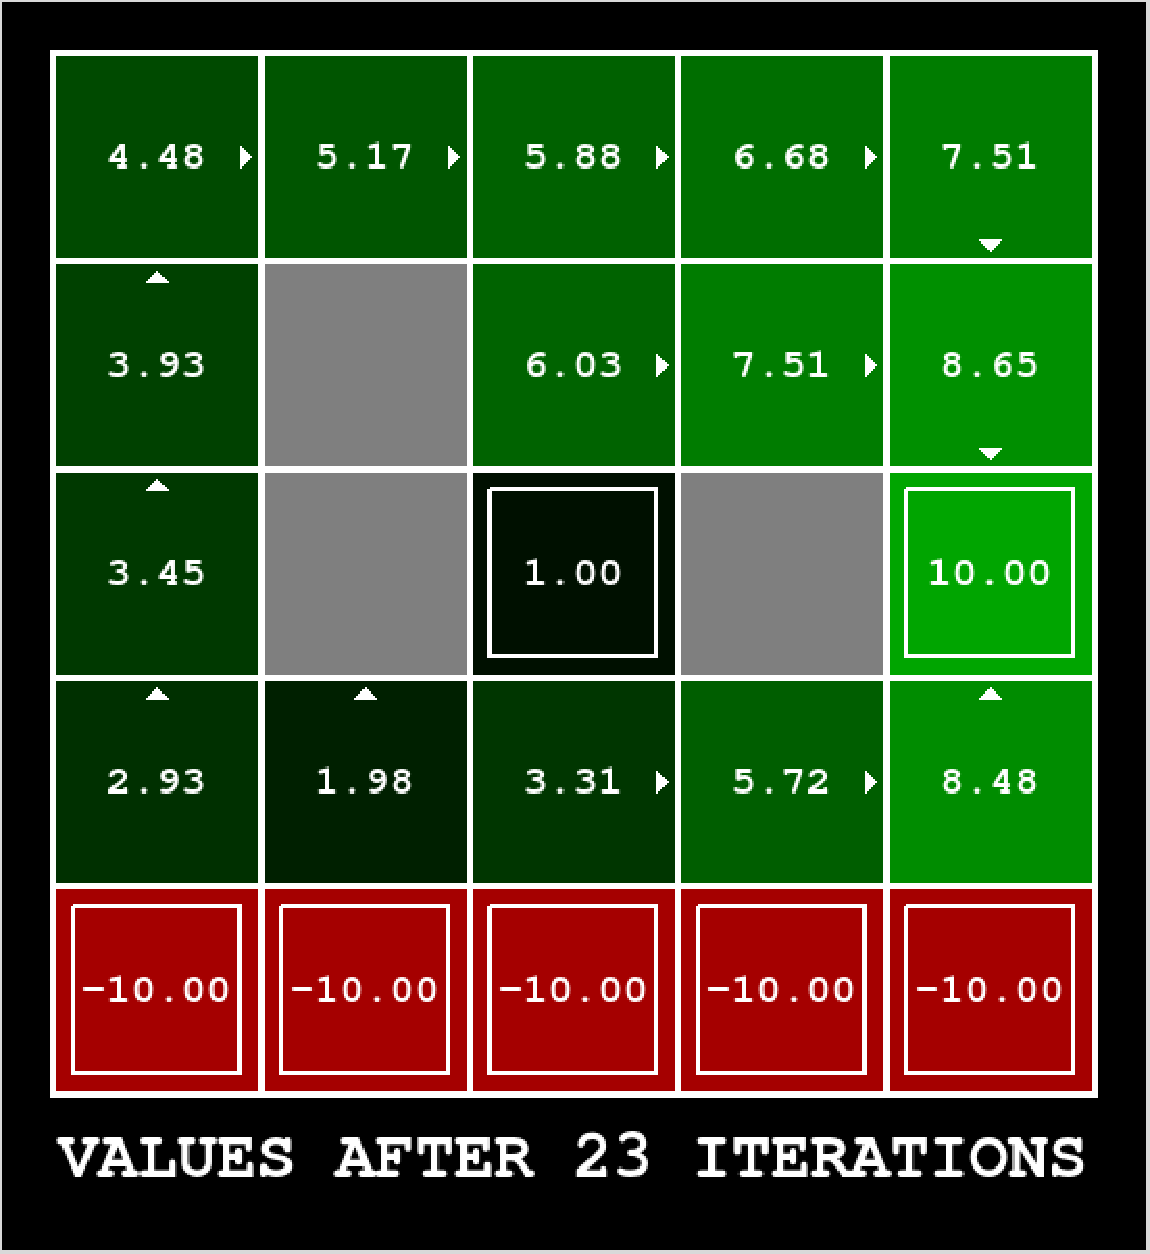
\includegraphics[width=1.5in]{images/discount/default.pdf}\label{discount-default}}~
    \subfloat[0.99]{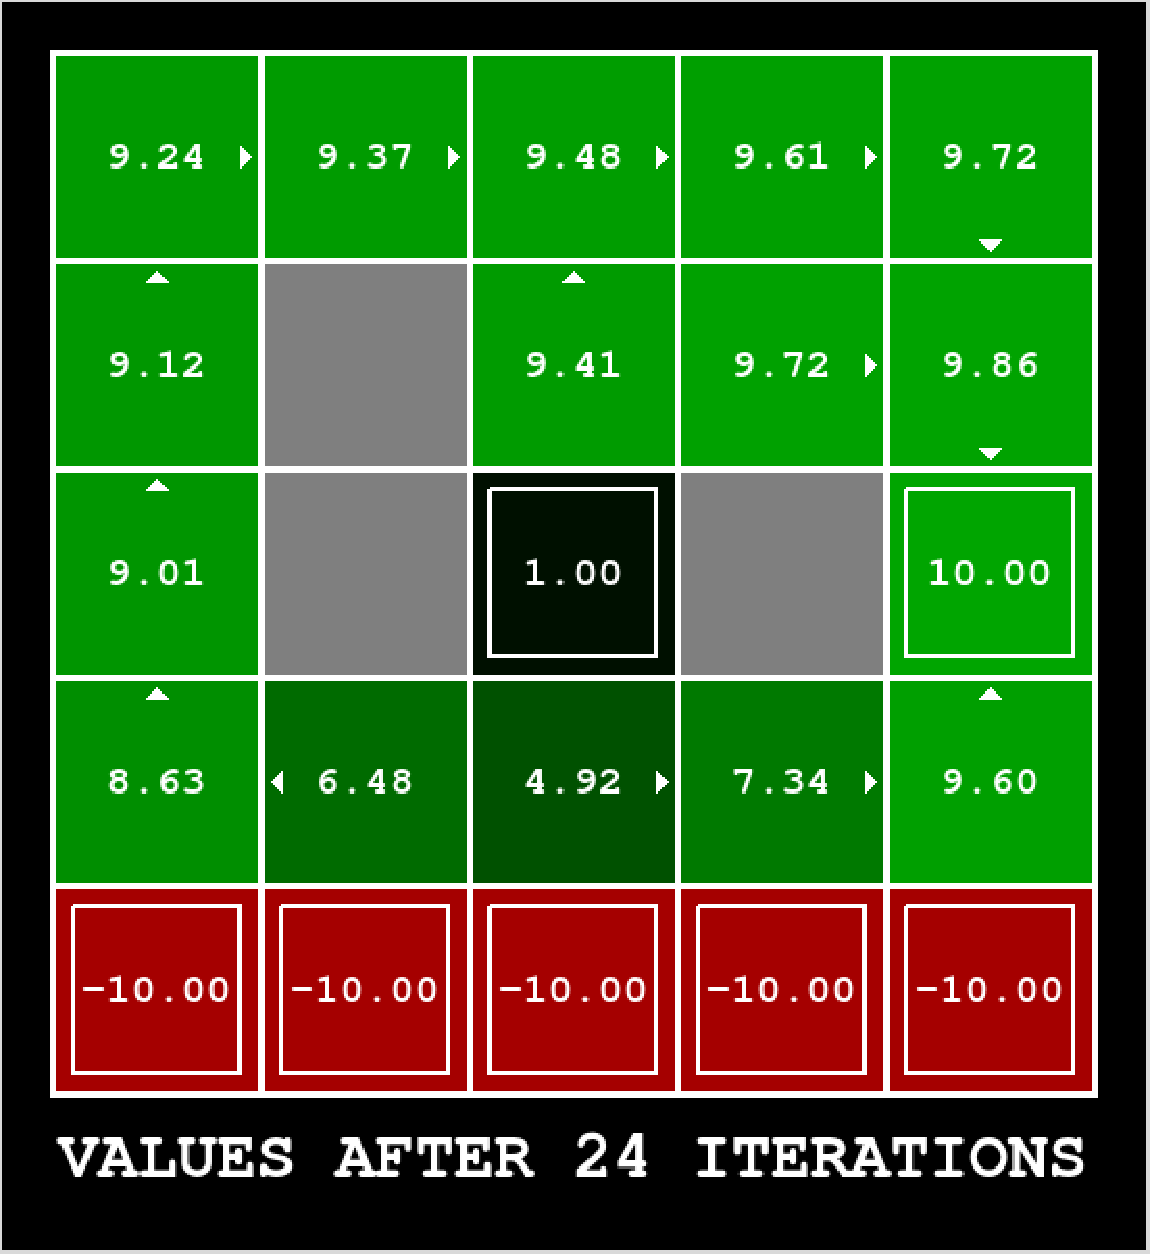
\includegraphics[width=1.5in]{images/discount/g-099.pdf}\label{discount-g099}}
    \caption{discount grid - various $\gamma$ settings}
\end{figure} 

\paragraph{Time matters}

With a $\gamma$ of 0.99, which reduces the effects of discounting, the policy shifts slightly (Figure~\ref{discount-g099}). The policy in state (2,2) now risks a direct movement to the east, given the higher expected utility of that action. This is due to the higher relative value of state (1,2) due to the reduced discounting. Also, state (3,6) avoids the risk of falling into the lower reward for the same reason. The expected value of attempting a northward movement is now relatively more valuable than with a move east policy, despite the indirect route to the terminal state. This shows the implications of adjusting delayed reward and how an agent could be lead to take greater risks or follow an otherwise sub-optimal route to gain a larger reward farther in the distance.

\paragraph{Rewards matter}

With a shift in rewards, we can affect how the resulting policy directs the agent. Figure~\ref{discount-r2} shows the result of changing the reward in all non-terminal states to -2. The policy now believes that the closer terminal state is a better alternative at state (3,2). The negative rewards, and risk of falling off the cliff, push the agent toward the closer end point. With the non-terminal rewards set to -3, this early termination policy extends to the northern path as well (Figure~\ref{discount-r3}). With a sufficiently negative non-terminal reward, we can even entice the agent to end the process as quickly as possible, by intentionally jumping off the cliff (Figure~\ref{discount-r11}).

\begin{figure}[!htbp]
    \centering
    \subfloat[-2]{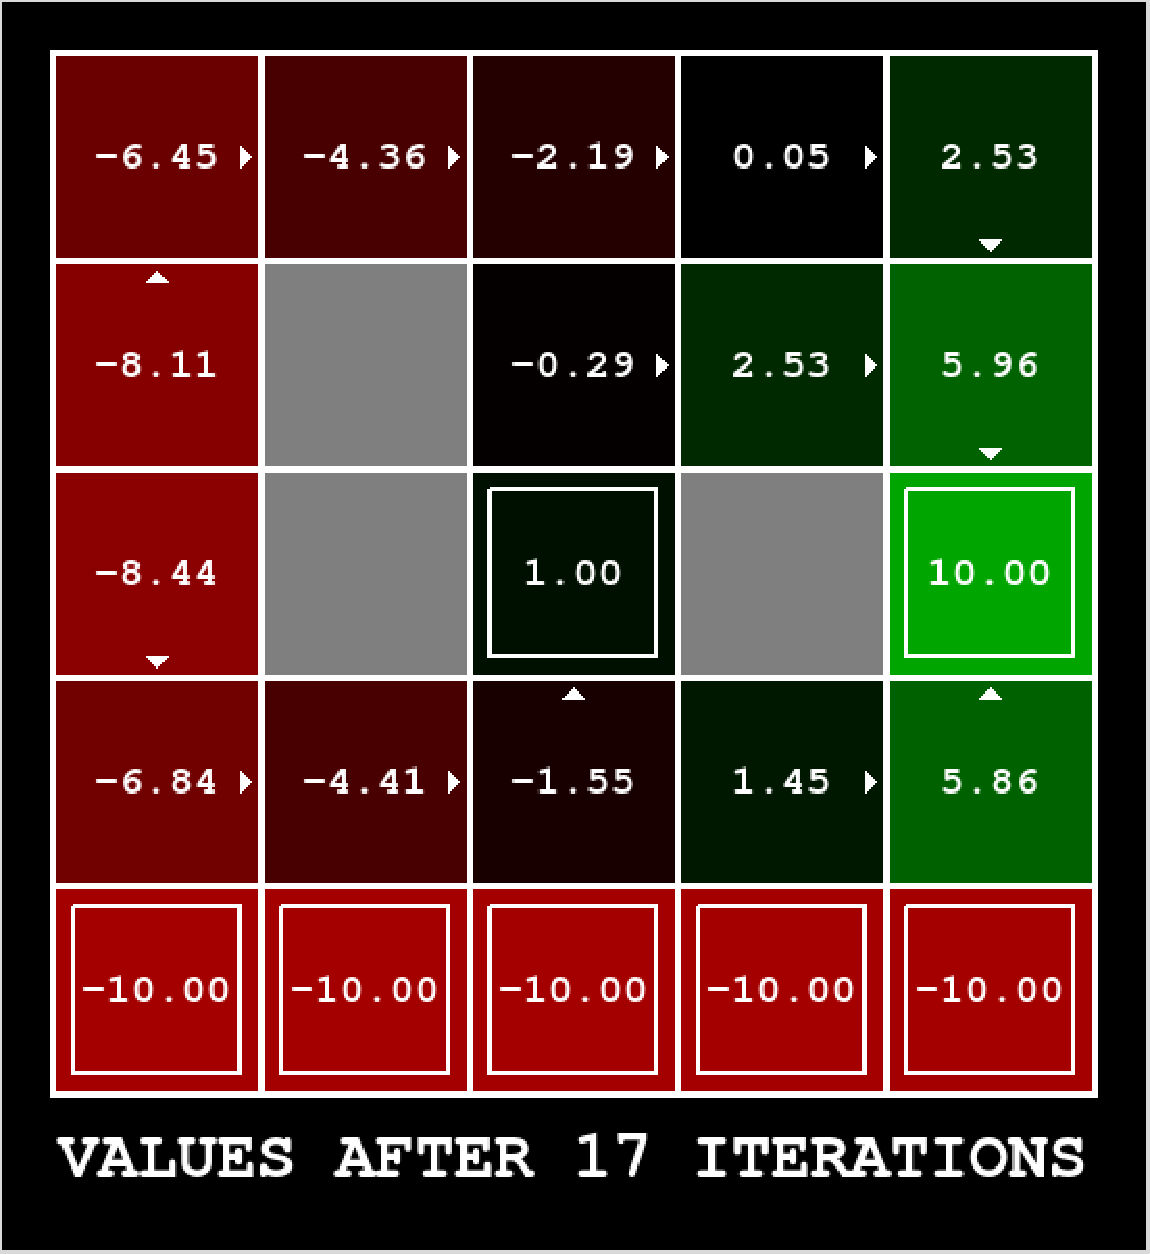
\includegraphics[width=1.5in]{images/discount/r-2.pdf}\label{discount-r2}}~
    \subfloat[-3]{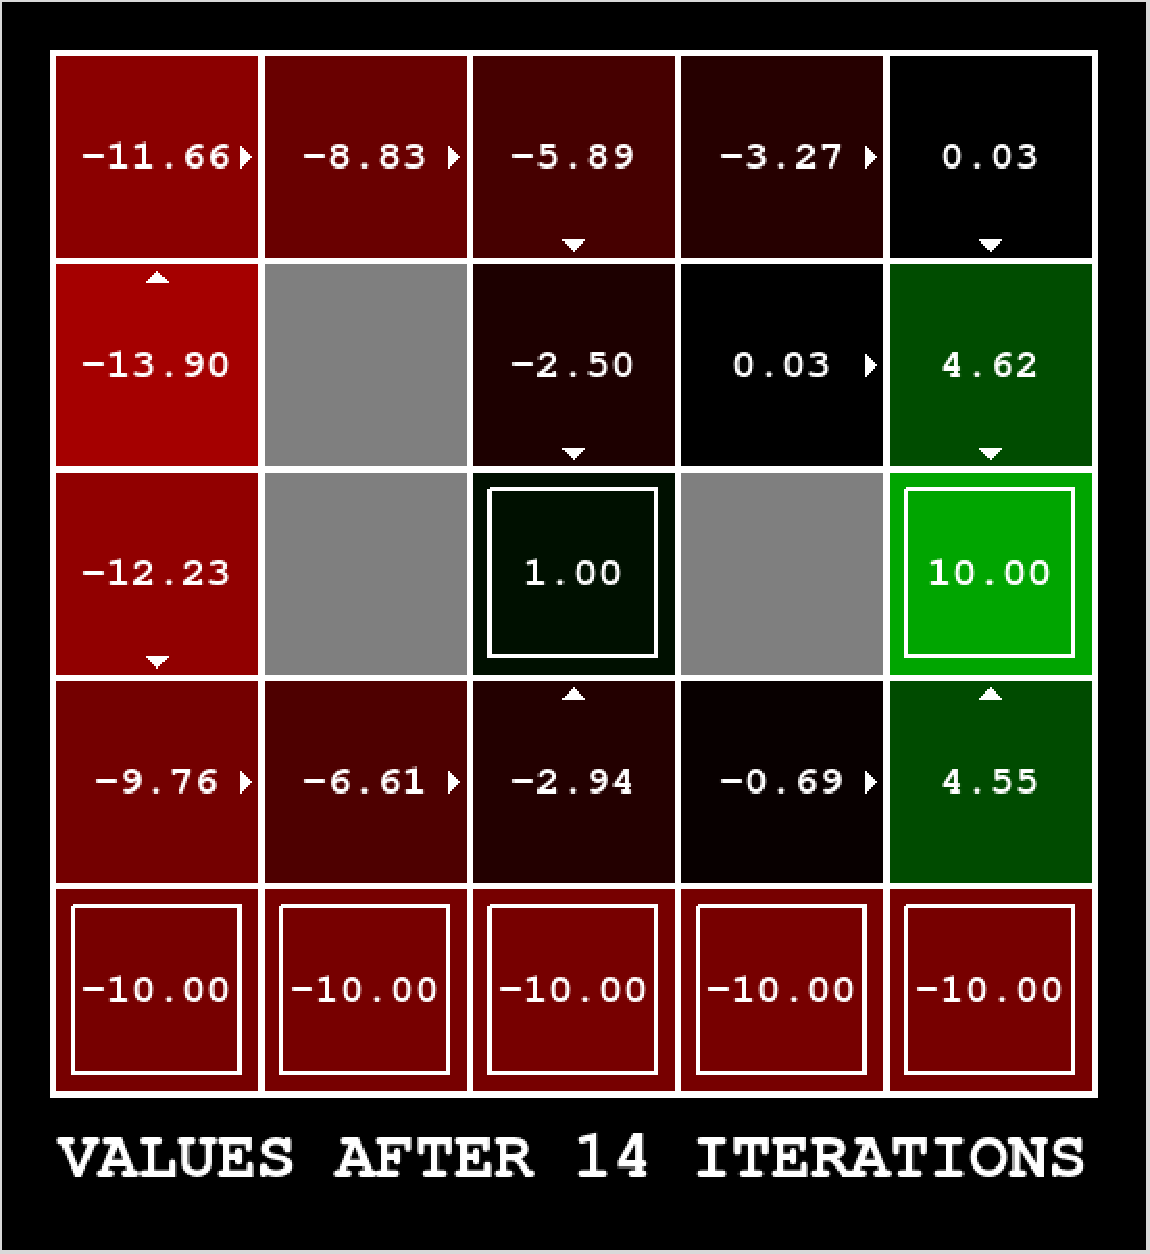
\includegraphics[width=1.5in]{images/discount/r-3.pdf}\label{discount-r3}}\\
    \subfloat[-11]{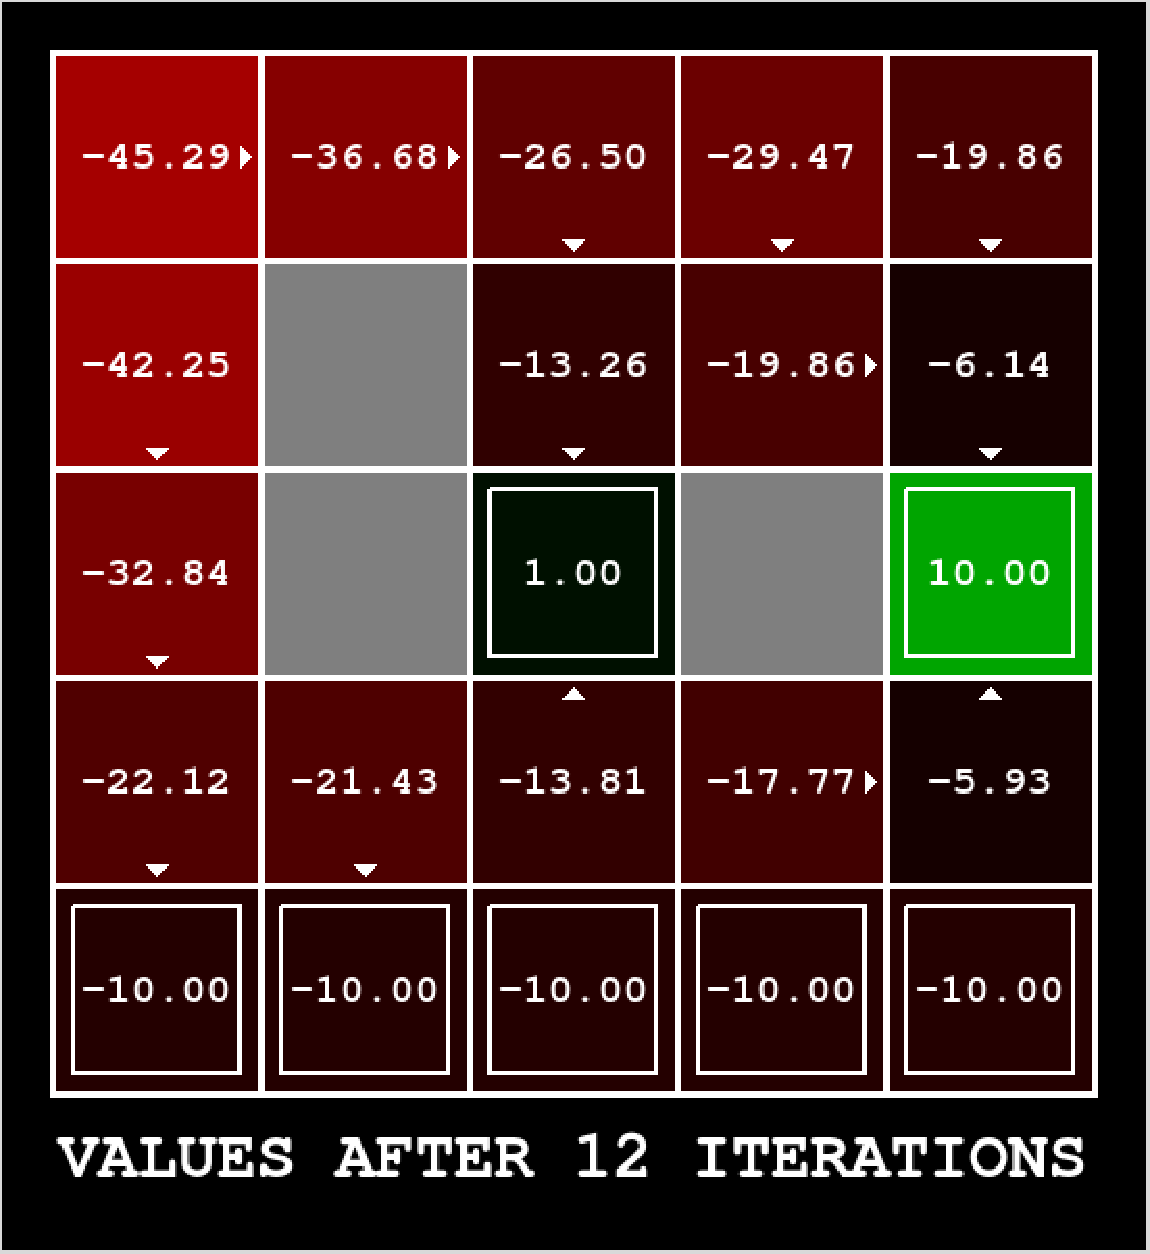
\includegraphics[width=1.5in]{images/discount/r-11.pdf}\label{discount-r11}}
    \caption{discount grid - various non-terminal reward settings}
\end{figure} 

\paragraph{The problem matters}

Policies are not only affected by planning algorithm parameters, but also by the problem definition, such as the probabilities in the transition function. If movement in the MDP is deterministic, or the intentional action probabilities are sufficiently high, otherwise risky paths would be considered optimal. Figure~\ref{discount-n001} shows a policy of cliff-walking given only a 1\% change of falling off the ledge. Conversely, the policy in Figure~\ref{discount-n04} shows how our planning algorithm would approach a high risk environment (inebriated agent). In the later case, the agent will avoid any east-west movement, even at the expense of exiting at the low reward terminal state.

\begin{figure}[!htbp]
    \centering
    \subfloat[0.01]{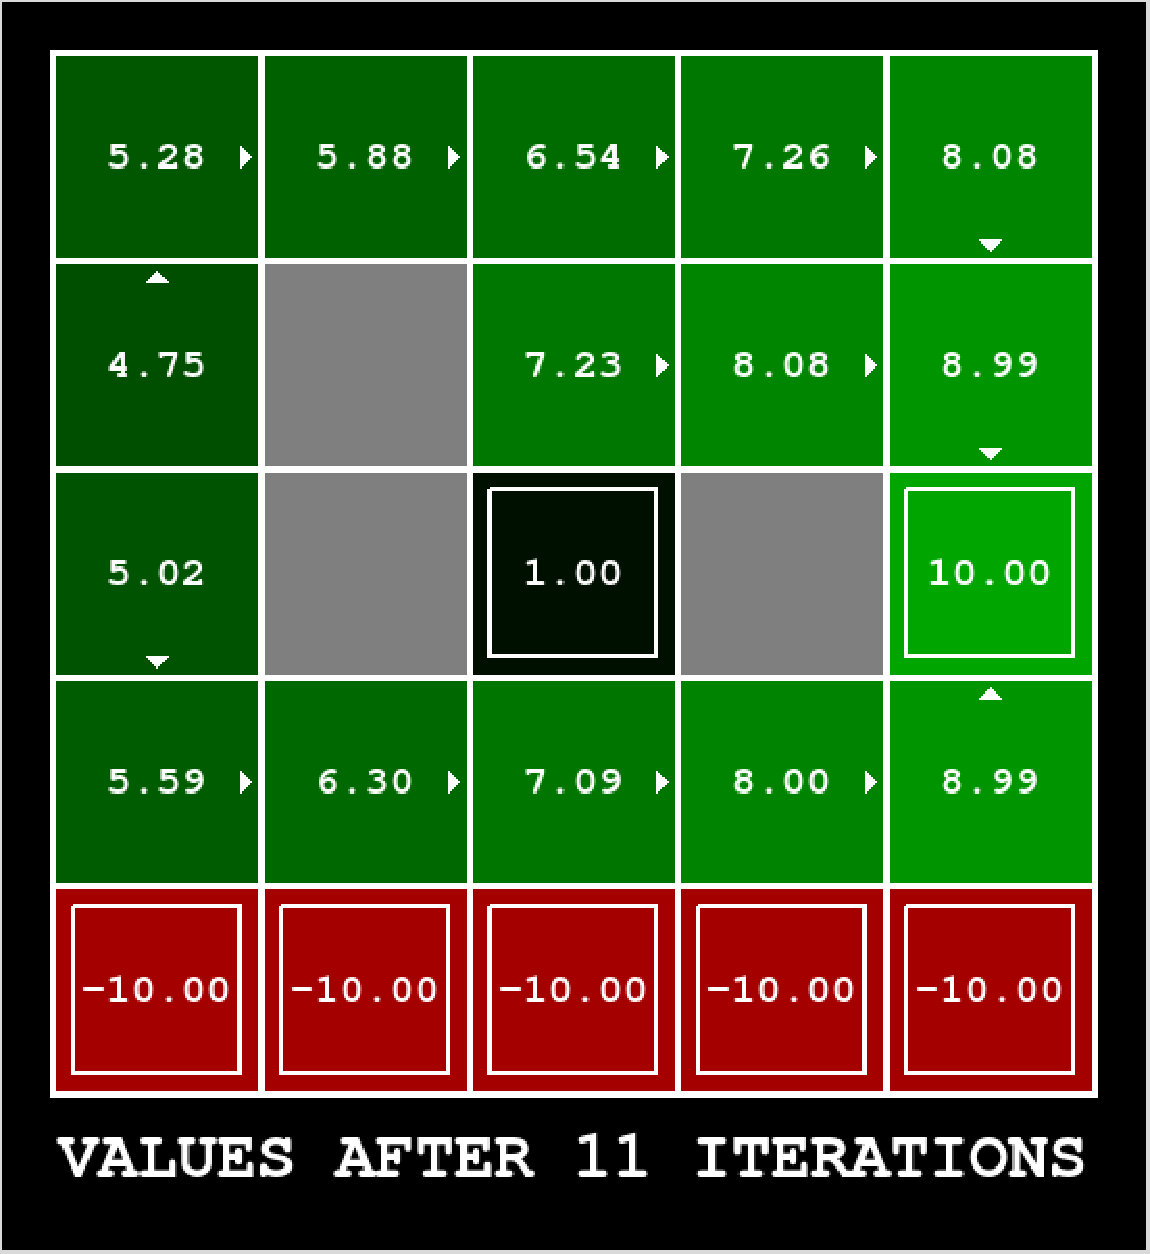
\includegraphics[width=1.5in]{images/discount/n-001.pdf}\label{discount-n001}}~
    \subfloat[0.4]{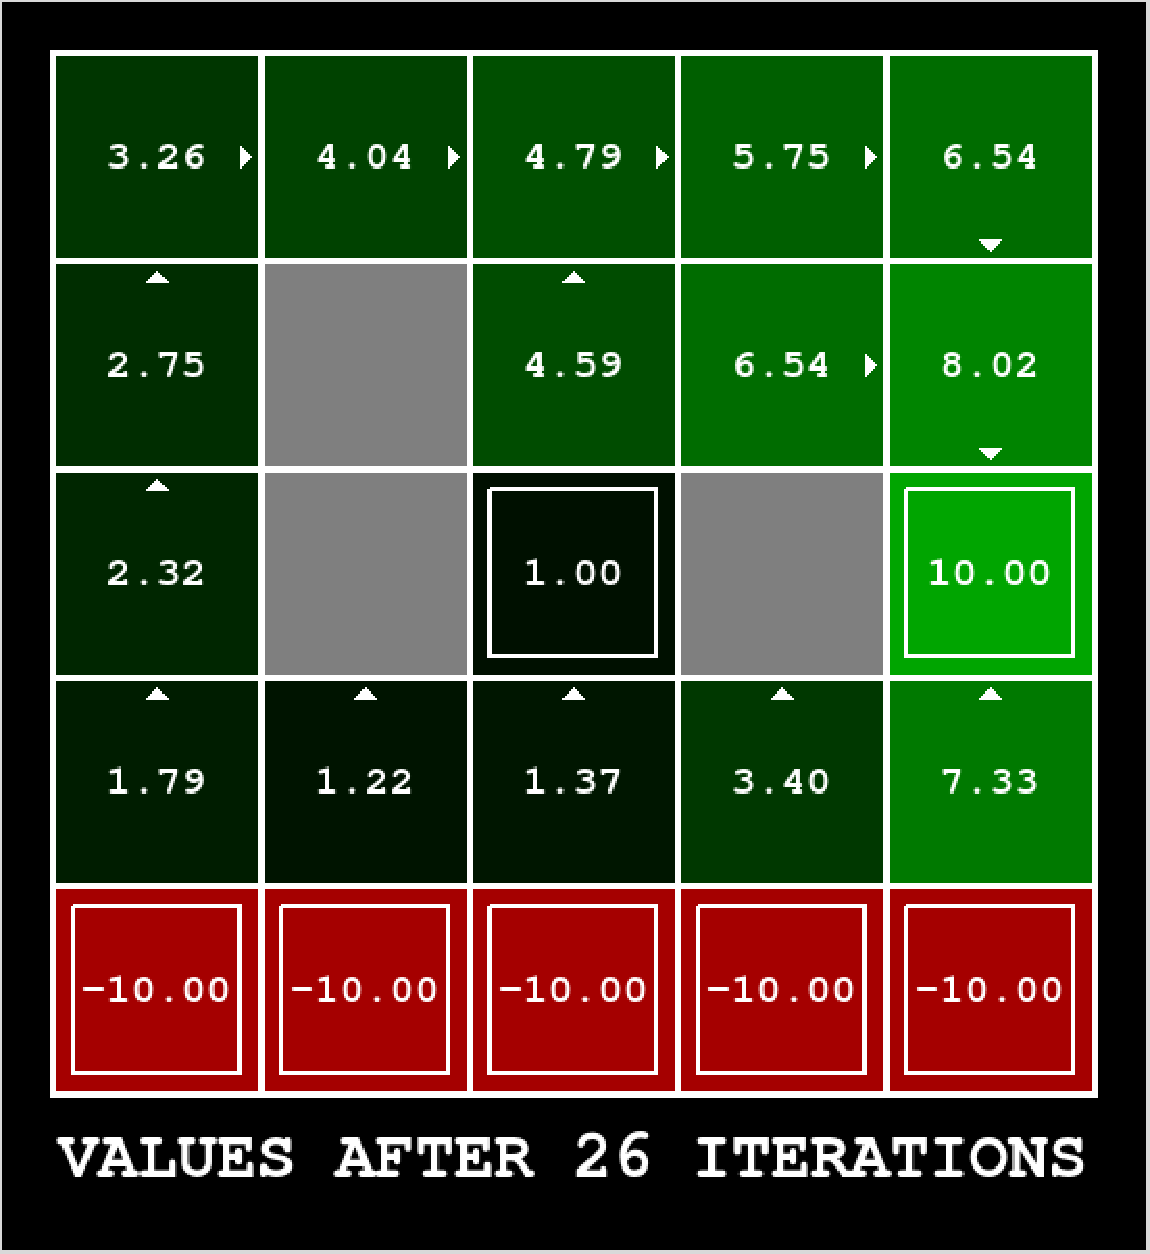
\includegraphics[width=1.5in]{images/discount/n-04.pdf}\label{discount-n04}}\\
    \caption{discount grid - various unintentional movement probabilities}
\end{figure} 

\subsection{Tunnel Grid}

Tunnel grid is a one dimensional grid with the starting state on one end and the only terminal state on the other. Although this grid is simplistic, it highlights the distinctions between our planning and learning algorithms well. For example, Figure~\ref{tunnel-performance} shows the elapsed time and the number of iterations/episodes each algorithm took to converge. In the case of Q-learning, an episode is determined as a single training run from the starting state until the agent reaches a terminal state.

\begin{figure}[!htbp]
    \centering
    \subfloat[value iteration]{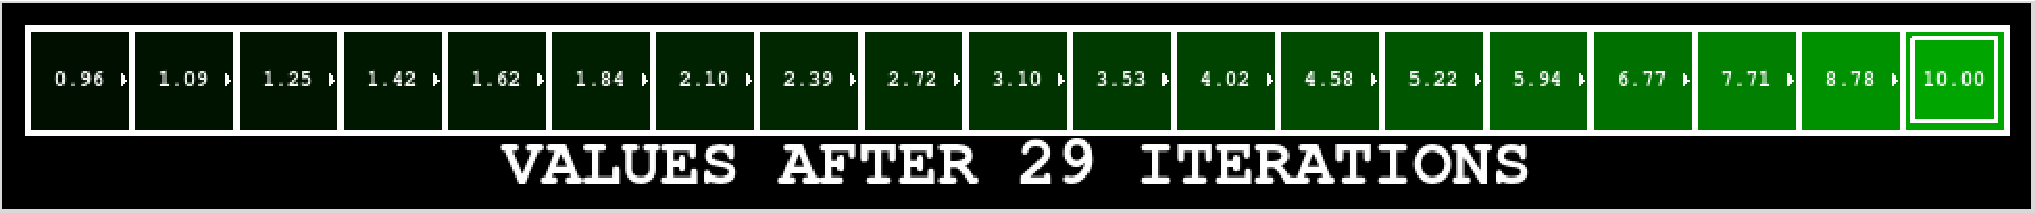
\includegraphics[width=3in]{images/tunnel/value.pdf}\label{tunnel-value}}\\
    \subfloat[policy iteration]{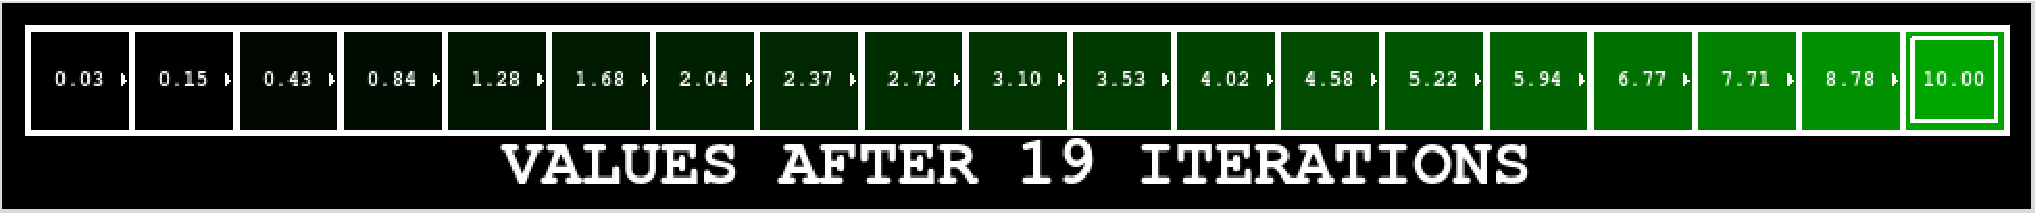
\includegraphics[width=3in]{images/tunnel/policy.pdf}\label{tunnel-policy}}\\
    \subfloat[q-learning]{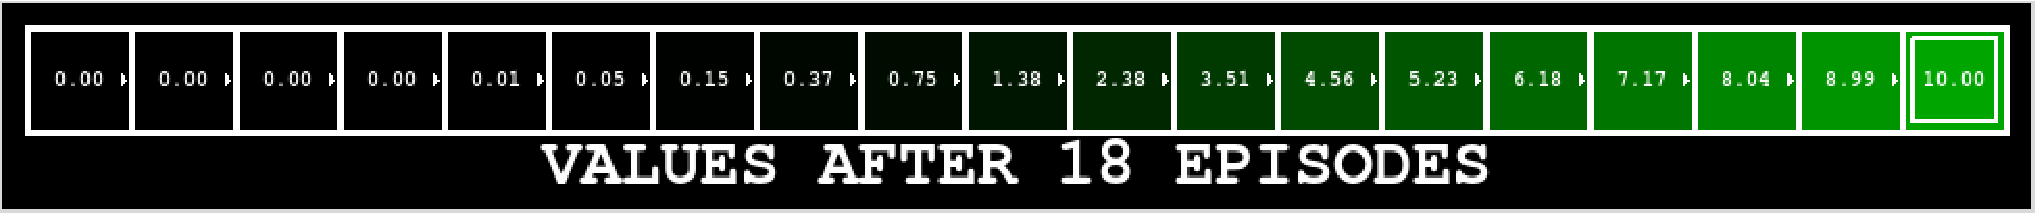
\includegraphics[width=3in]{images/tunnel/q.pdf}\label{tunnel-q}}
    \caption{tunnel grid}
\end{figure} 


    \begin{table}[h]
    \begin{tabular}{lllll}
               & Elapsed Time & Iterations/Episodes &  &  \\
    Value      & 0.04         & 29                  &  &  \\
    Policy     & 0.04         & 19                  &  &  \\
    Q-Learning & 0.390        & 18                  &  & 
    \end{tabular}
    \caption{tunnel grid - performance\label{tunnel-performance}}
    \end{table}

\section{Value Iteration}


\section{Policy Iteration}

\section{Q-Learning}

metrics
    elapsed time
    hamming distance

lazy vs. eager learning.

planning performance

policy iteration implementation issues
    get's stuck with only policy change check
    takes too long with epsilon check
    works well with value update check


q-learning performnace
q-learning strategies








\bibliographystyle{abbrv}
\bibliography{references}


\end{document}
